% Options for packages loaded elsewhere
% Options for packages loaded elsewhere
\PassOptionsToPackage{unicode}{hyperref}
\PassOptionsToPackage{hyphens}{url}
\PassOptionsToPackage{dvipsnames,svgnames,x11names}{xcolor}
%
\documentclass[
  11pt,
  letterpaper,
  DIV=11,
  numbers=noendperiod]{scrartcl}
\usepackage{xcolor}
\usepackage[top=0.75in,left=0.75in,bottom=0.75in,right=0.75in]{geometry}
\usepackage{amsmath,amssymb}
\setcounter{secnumdepth}{3}
\usepackage{iftex}
\ifPDFTeX
  \usepackage[T1]{fontenc}
  \usepackage[utf8]{inputenc}
  \usepackage{textcomp} % provide euro and other symbols
\else % if luatex or xetex
  \usepackage{unicode-math} % this also loads fontspec
  \defaultfontfeatures{Scale=MatchLowercase}
  \defaultfontfeatures[\rmfamily]{Ligatures=TeX,Scale=1}
\fi
\usepackage{lmodern}
\ifPDFTeX\else
  % xetex/luatex font selection
\fi
% Use upquote if available, for straight quotes in verbatim environments
\IfFileExists{upquote.sty}{\usepackage{upquote}}{}
\IfFileExists{microtype.sty}{% use microtype if available
  \usepackage[]{microtype}
  \UseMicrotypeSet[protrusion]{basicmath} % disable protrusion for tt fonts
}{}
\makeatletter
\@ifundefined{KOMAClassName}{% if non-KOMA class
  \IfFileExists{parskip.sty}{%
    \usepackage{parskip}
  }{% else
    \setlength{\parindent}{0pt}
    \setlength{\parskip}{6pt plus 2pt minus 1pt}}
}{% if KOMA class
  \KOMAoptions{parskip=half}}
\makeatother
% Make \paragraph and \subparagraph free-standing
\makeatletter
\ifx\paragraph\undefined\else
  \let\oldparagraph\paragraph
  \renewcommand{\paragraph}{
    \@ifstar
      \xxxParagraphStar
      \xxxParagraphNoStar
  }
  \newcommand{\xxxParagraphStar}[1]{\oldparagraph*{#1}\mbox{}}
  \newcommand{\xxxParagraphNoStar}[1]{\oldparagraph{#1}\mbox{}}
\fi
\ifx\subparagraph\undefined\else
  \let\oldsubparagraph\subparagraph
  \renewcommand{\subparagraph}{
    \@ifstar
      \xxxSubParagraphStar
      \xxxSubParagraphNoStar
  }
  \newcommand{\xxxSubParagraphStar}[1]{\oldsubparagraph*{#1}\mbox{}}
  \newcommand{\xxxSubParagraphNoStar}[1]{\oldsubparagraph{#1}\mbox{}}
\fi
\makeatother


\usepackage{longtable,booktabs,array}
\usepackage{calc} % for calculating minipage widths
% Correct order of tables after \paragraph or \subparagraph
\usepackage{etoolbox}
\makeatletter
\patchcmd\longtable{\par}{\if@noskipsec\mbox{}\fi\par}{}{}
\makeatother
% Allow footnotes in longtable head/foot
\IfFileExists{footnotehyper.sty}{\usepackage{footnotehyper}}{\usepackage{footnote}}
\makesavenoteenv{longtable}
\usepackage{graphicx}
\makeatletter
\newsavebox\pandoc@box
\newcommand*\pandocbounded[1]{% scales image to fit in text height/width
  \sbox\pandoc@box{#1}%
  \Gscale@div\@tempa{\textheight}{\dimexpr\ht\pandoc@box+\dp\pandoc@box\relax}%
  \Gscale@div\@tempb{\linewidth}{\wd\pandoc@box}%
  \ifdim\@tempb\p@<\@tempa\p@\let\@tempa\@tempb\fi% select the smaller of both
  \ifdim\@tempa\p@<\p@\scalebox{\@tempa}{\usebox\pandoc@box}%
  \else\usebox{\pandoc@box}%
  \fi%
}
% Set default figure placement to htbp
\def\fps@figure{htbp}
\makeatother





\setlength{\emergencystretch}{3em} % prevent overfull lines

\providecommand{\tightlist}{%
  \setlength{\itemsep}{0pt}\setlength{\parskip}{0pt}}



 


\KOMAoption{captions}{tableheading}
\usepackage{hyperref}
\newenvironment{customabstract}{ \begin{center} {\bfseries Abstract}\par\vspace{0.5em} \begin{minipage}{0.8\linewidth} }{ \end{minipage} \end{center} }
\makeatletter
\@ifpackageloaded{caption}{}{\usepackage{caption}}
\AtBeginDocument{%
\ifdefined\contentsname
  \renewcommand*\contentsname{Table of contents}
\else
  \newcommand\contentsname{Table of contents}
\fi
\ifdefined\listfigurename
  \renewcommand*\listfigurename{List of Figures}
\else
  \newcommand\listfigurename{List of Figures}
\fi
\ifdefined\listtablename
  \renewcommand*\listtablename{List of Tables}
\else
  \newcommand\listtablename{List of Tables}
\fi
\ifdefined\figurename
  \renewcommand*\figurename{Figure}
\else
  \newcommand\figurename{Figure}
\fi
\ifdefined\tablename
  \renewcommand*\tablename{Table}
\else
  \newcommand\tablename{Table}
\fi
}
\@ifpackageloaded{float}{}{\usepackage{float}}
\floatstyle{ruled}
\@ifundefined{c@chapter}{\newfloat{codelisting}{h}{lop}}{\newfloat{codelisting}{h}{lop}[chapter]}
\floatname{codelisting}{Listing}
\newcommand*\listoflistings{\listof{codelisting}{List of Listings}}
\makeatother
\makeatletter
\makeatother
\makeatletter
\@ifpackageloaded{caption}{}{\usepackage{caption}}
\@ifpackageloaded{subcaption}{}{\usepackage{subcaption}}
\makeatother
\usepackage{bookmark}
\IfFileExists{xurl.sty}{\usepackage{xurl}}{} % add URL line breaks if available
\urlstyle{same}
\hypersetup{
  pdftitle={Diamonds},
  pdfauthor={Prera \& Agrawal},
  colorlinks=true,
  linkcolor={blue},
  filecolor={Maroon},
  citecolor={purple},
  urlcolor={purple},
  pdfcreator={LaTeX via pandoc}}


\title{Diamonds}
\author{Prera \& Agrawal}
\date{}
\begin{document}
\maketitle

\renewcommand*\contentsname{Contents}
{
\hypersetup{linkcolor=blue}
\setcounter{tocdepth}{3}
\tableofcontents
}

\newpage

\begin{customabstract}
This is my abstract
\end{customabstract}

\newpage

\section{Introduction}\label{introduction}

\section{Exploratory Data Analysis}\label{exploratory-data-analysis}

\begin{figure}[H]

\centering{

\pandocbounded{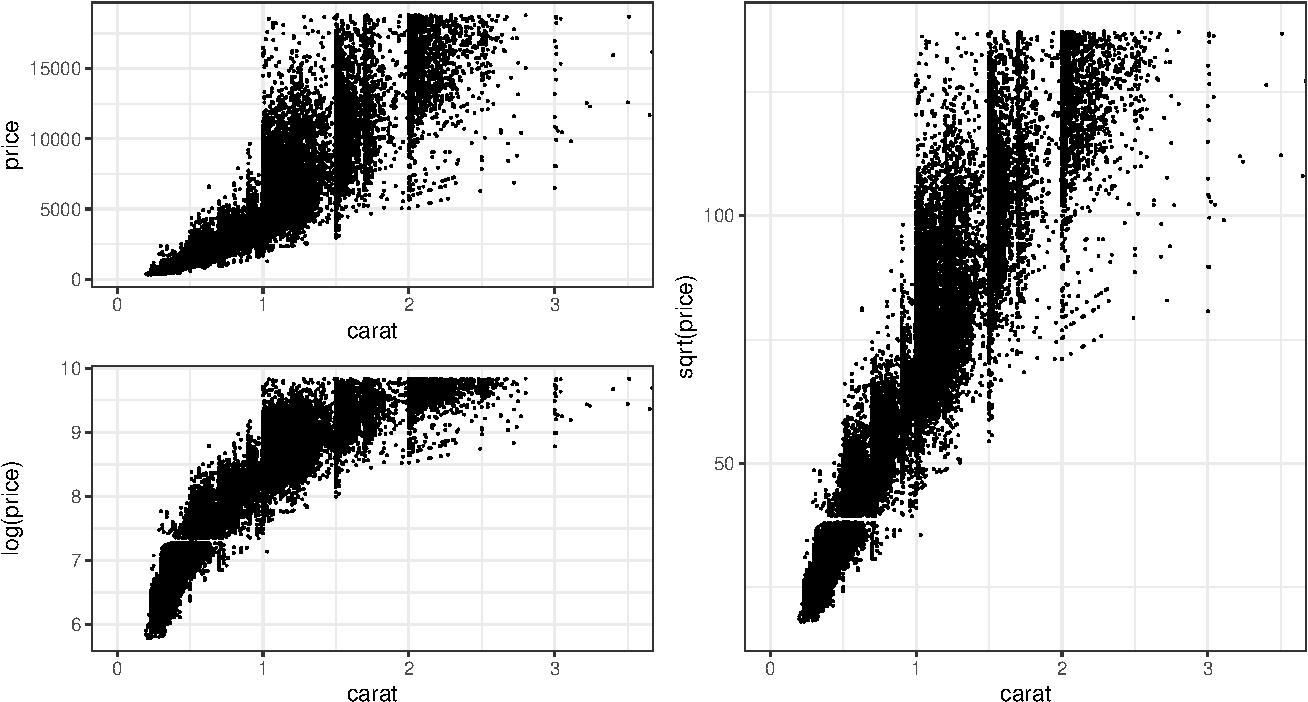
\includegraphics[keepaspectratio]{MTH-245-Project-QMD-Starter-File_files/figure-pdf/fig-price-vs-diamond-1.pdf}}

}

\caption{\label{fig-price-vs-diamond}Price vs Diamonds}

\end{figure}%

Firstly, we tried to understand the relationship of Diamond prices with
the predictors we have in the dataset. The first obvious predictor to
consider was carats, as popularized by advertisements on the Fifth
Avenue by De Beers, ``Bigger is Better.'' (Cite the book Many Meanings
of Diamonds, Susan Falls) We guessed initially that it would not be a
linear relationship, thus, we immediately applied a logarithmic
transformation. To our dismay, the graph just looked reflected and after
an hour of other forms of data exploration, we tried applying a square
root transformation, and the graph became immediately linear.

\begin{figure}[H]

\centering{

\pandocbounded{\includegraphics[keepaspectratio]{MTH-245-Project-QMD-Starter-File_files/figure-pdf/fig-price-vs-volume-1.pdf}}

}

\caption{\label{fig-price-vs-volume}Price vs volume}

\end{figure}%

Maybe talk about how the slopes compare to each other. The first volume
graph is obvious, but the difference between the slopes of the other 3
seems to be quite different. Which means with growing depth, the diamond
price increases faster as compared to the increase in length or width.

Apart from that, it is pretty fascinating that the price is just
correlated exponentially with the volume, and thus also exponentially
with the rest of the items.

If we were to strictly stick to a linear regression, we should not be
caring about x, y, and z, we may lose some information but we need to
use volume because we cannot cube the x, y, and z.

\begin{figure}[H]

\centering{

\pandocbounded{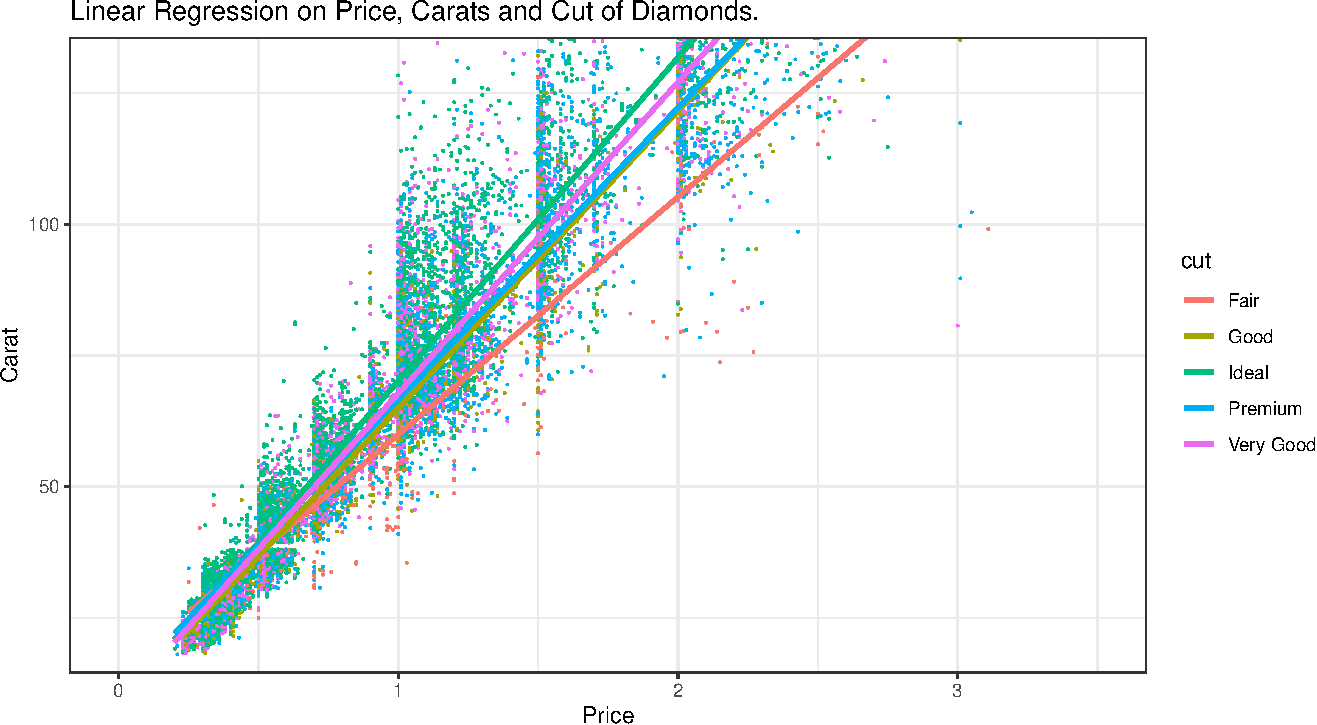
\includegraphics[keepaspectratio]{MTH-245-Project-QMD-Starter-File_files/figure-pdf/fig-price-vs-diamond-vs-cut-1.pdf}}

}

\caption{\label{fig-price-vs-diamond-vs-cut}Price vs Diamonds}

\end{figure}%

\begin{figure}[H]

\centering{

\pandocbounded{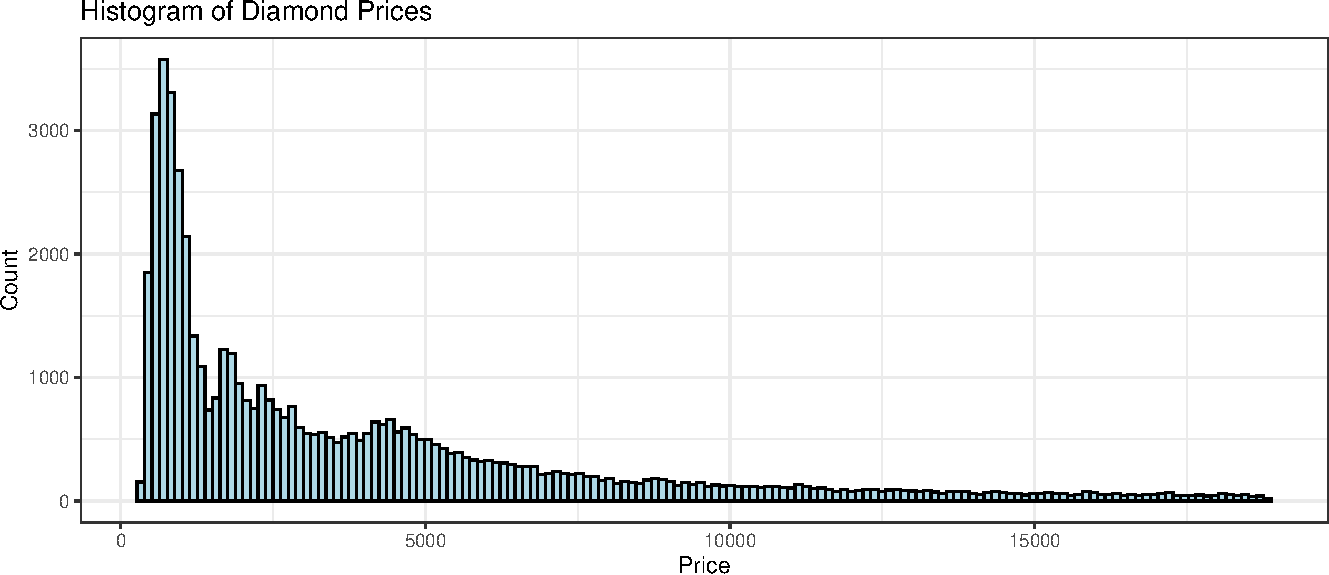
\includegraphics[keepaspectratio]{MTH-245-Project-QMD-Starter-File_files/figure-pdf/fig-prices-hist-1.pdf}}

}

\caption{\label{fig-prices-hist}Histogram of Diamond Prices.}

\end{figure}%

\begin{verbatim}
<ggplot2::labels> List of 3
 $ x    : chr "depth"
 $ y    : chr "price"
 $ title: chr "Histogram of Diamond Prices vs depth"
\end{verbatim}

\begin{figure}[H]

\centering{

\pandocbounded{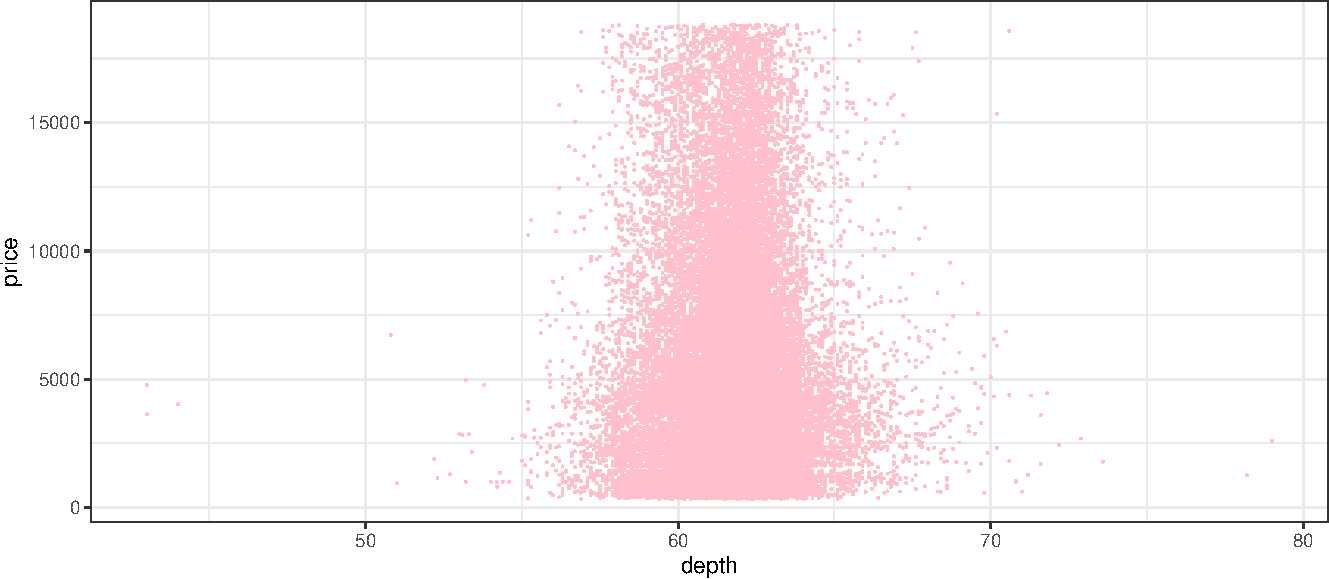
\includegraphics[keepaspectratio]{MTH-245-Project-QMD-Starter-File_files/figure-pdf/fig-prices-depth-scatt-1.pdf}}

}

\caption{\label{fig-prices-depth-scatt}Histogram of Diamond depth and
price}

\end{figure}%

\section{Methods}\label{methods}

Figure~\ref{fig-price-vs-diamond}

\section{Conclusion}\label{conclusion}

\section{References}\label{references}




\end{document}
